\documentclass{article}
\usepackage[utf8]{inputenc}
\usepackage{graphicx}

% change reference style to [1], remove stupid sorting, language changed so date in ddmmyyyy
\usepackage[backend=biber, style=numeric, sorting=none, language=australian]{biblatex}
\addbibresource{References.bib}

\title{Detecting User Engagement Using \\ Mouse Tracking Data:\\
    \large Project Specification
}
\author{David Saunders (910995)}
\date{April 2020}

\begin{document}
\maketitle

\begin{abstract} 
    Write abstract here
\end{abstract}

\tableofcontents

% \section*{Mark scheme}
% This coursework contributes 50\% of the mark for the module. The size is
% approximately 5000 words (excluding references) – due on Wednesday 29
% April 2020 (11:00 am).

% This report should give a literature review over your project and describe
% any background research that you have carried out. 
% You should state the motivation and aims of the project. 
% It should include a complete specification of your project. 
% It should describe the project clearly and the components
% of the work which need to be developed. 
% An outline project plan for the summer should be included. 
% This plan should take into account the development methodology being used. 
% You should provide a risk analysis for the project. 
% You should view this document as providing the plan for the work
% you expect to carry out over the summer.

% TO SUMMARISE The structure POINTS
% - Literature Review
%   - Background research
% - Motivation and aims of Project
%   - Clearly describe project and components 
% - Outline Project Plan
%   - Include methodology used. 
% - Risk Analysis


% \begin{figure}[ht]
%     \centering
%     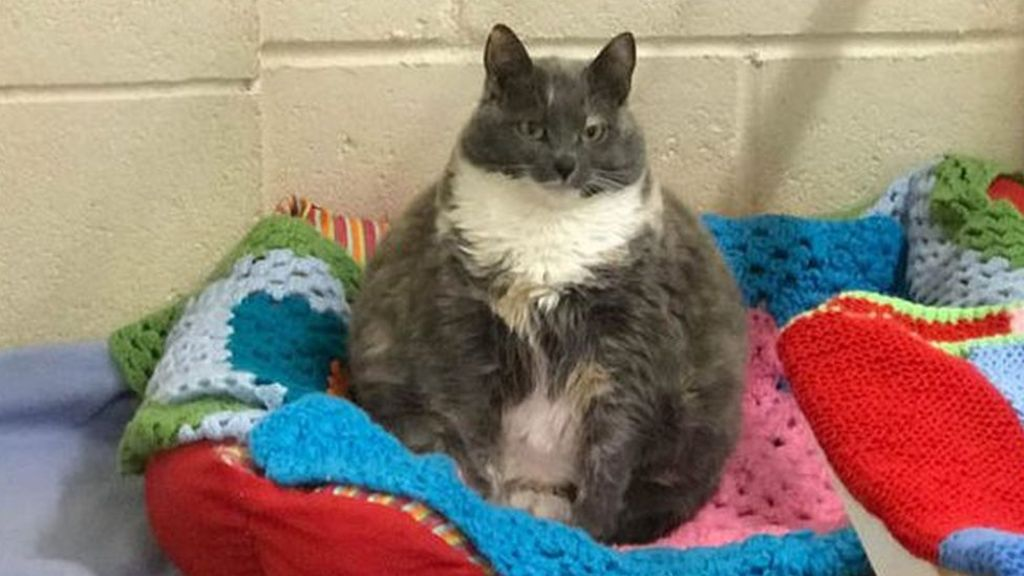
\includegraphics[scale=0.35]{Test.JPG}
%     \caption{This will be a figure showcasing some of my work}
%     \label{fig:test}
% \end{figure}
% Write section 1 here \cite{torsney2011tuner} and talk about figure \ref{fig:test}.

\section{Literature review}

In this section I will review the literature on how to monitor attention.

%This can pretty much be the review I did for the first assignment. 

\section{Background Research}
Anything I've looked at with help for mouse data classification algorithms? 


\section{Motivation and Aims of project}
Can copy from presentation slides but fill in so they're more wordy.

\subsection{Motivation}

People are lazy. 
Often don't pay much attention 
Is there any way of measuring people's attention?

Why mouse data?
Mouse cursor position is strongly correlated with eye position. 
One paper calls it a “poor man's eye-tracker” [find]
Bulky expensive equipment for eye tracking is expensive and very obtrusive.
Hawthorn / observer effect - People react differently when being observed. 
Less obtrusive mouse tracking can make people feel less tracked and act more naturally. 
Could even not tell them (legal ethical repercussions)!

\subsection{Aims of project}

The aims of what I want to achieve in the project will be as follows:
\begin{itemize}
    \item Visualise, analyse and understand the data results.
    \item Use the data to train machine learning models to classify users between 2 groups.
    \item Combine the data and methods from the study data with other datasets to create a more robust model.
    \item Stretch goal? Test methods and models developed with other applications?
\end{itemize}

Talk here about how I will achieve each aim, then describe the components of the project that I will need to complete.
Try and link each component of the project to an aim.

Machine learning methods
    SVM
    Natural Language Processing
    N-Grams
    LSTM Neural Networks
    Markov models
Deal with Imbalances in classes
    Sampling
    Oversampling, Undersampling
Other mouse data sources

Applications
A good system developed could be used for other tasks to monitor attention - E.g. Survey Monika made us do. Not just for joes ice-cream
Have to decide on the trade off between a good narrow (is this the right word) classifier between attention or not and a more generalised model that can work on any task.
What I mean by that is I can model the html elements / sliders to see how users interacted to see the stock prices, or I can generalise to any such task involving mouse data.

\section{Project plan}

\subsection{Development methodology}
Discuss software life cycle methodologies with Jacques.
An agile methodology such as scrum would probably be best but am I constrained  by this specification document?

\begin{figure}[ht]
    \centering
    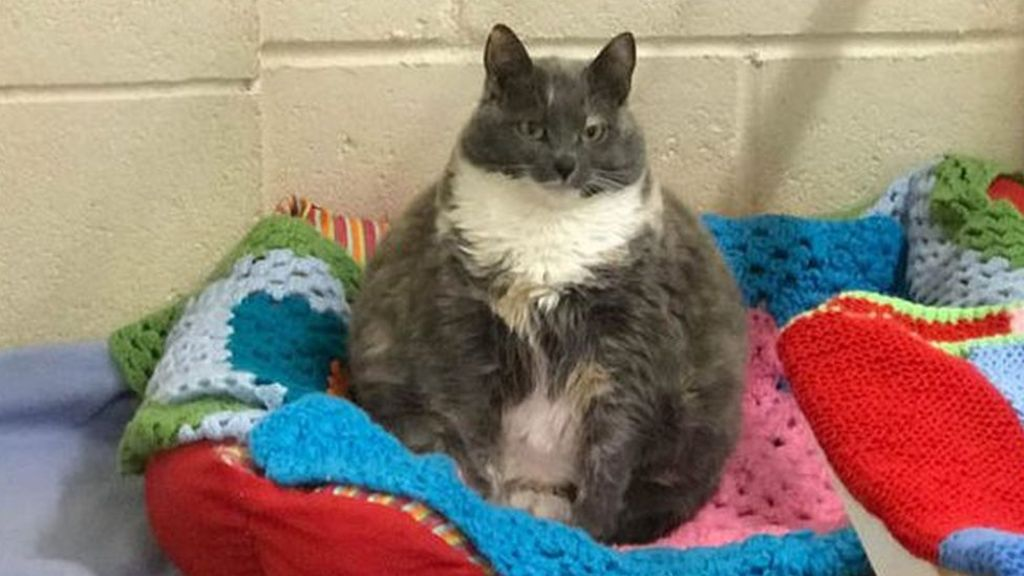
\includegraphics[scale=0.35]{Test.JPG}
    \caption{A Gantt chart showing the planned milestones of the project. OR A Gantt chart created in the GanttProject free software}
    \label{fig:Gantt}
\end{figure}

\section{Risk Analysis}
% Copy risk analysis from last year.
When creating a project there is always potential risks that the project might encounter and hinder its chances of success. 
In order to prepare and to hopefully avoid these risks I will now list and analyse the most likely, and most devastating risks to my project. 
By analysing each risk individually I will be prepared in case I come across any of the potential risks and I will have developed a plan of action of what to do and how to manage myself in case of encountering them. 
I will initially list the risks in a table where I will briefly examine them, then I will go into each one in more detail. 
Below I have listed and analysed the risks and have ordered them from potentially the most dangerous to least dangerous. 

Caption A risk analysis table
DAAAAAAAAAAAAAAAAAVE

% Please add the following required packages to your document preamble:
% \usepackage[table,xcdraw]{xcolor}
% If you use beamer only pass "xcolor=table" option, i.e. \documentclass[xcolor=table]{beamer}

\begin{table}[ht]
    \small %small not needed
    \caption{\label{table:individual} The top association rules between individual items.}
    \makebox[\textwidth][c]{%
        \begin{tabular}{|p{2cm}|p{1cm}|p{1cm}|p{1cm}|p{2cm}|p{2cm}|}
            \hline 
            { Risk}                                                                                                       & { Probability} & { Impact} & { Combined Risk} & { Mitigation Plan}                                                                                               & { Contingency Plan}                                                                                                                  \\
            { Unrealistic time   plan and poor time management.}                                                          & { High}        & { High}   & { High}          & { Create work   schedule and stick to it.}                                                                       & { If I am unable to   stick to my work schedule, I must adapt my approach to work and create an   undated, more realistic schedule.} \\
            { Coronavirus   affects me or a close family member, negatively effecting my work.}                           & { Medium}      & { High}   & { High}          & { Stay   safe during the quarantine to keep everyone safe and mitigate any risks of me   catching anything.}     & { Inform   the University as soon as a situation develops so we can arrange something.}                                              \\
            { Coronavirus   has a greater impact on Swansea University and  effects the available support and deadlines.} & { Medium}      & { High}   & { Medium}        & { Keep   informed with the University College of Science and supervisor to any news   effecting the University.} & { Keep my   options open? Keep updated?}                                                                                             \\
            { No correlation   between attention and mouse tracking data can be found.}                                   & { Low}         & { High}   & { Medium}        & { Attempt   as many different methods of classification early before writing in depth about   them.}             & { If no   insights can be gained from the given dataset, I will attempt to find   correlations in other datasets.}                   \\                                                                                                                    
        \end{tabular}
    }
\end{table}

\section{Conclusion}

Measuring user engagement is challenging
Mouse data can help us solve that issue by showing user attention
Data Science techniques could be used to help classify the data (Not SVM)


\printbibliography

\end{document}